\documentclass[11pt]{article}

\usepackage[margin=1in]{geometry}
\usepackage{amsmath,amssymb,mathtools}
\usepackage{booktabs}
\usepackage{graphicx}
\usepackage[font=small,labelfont=bf]{caption}
\usepackage{array}
\usepackage{hyperref}
\usepackage{microtype}
\usepackage{siunitx}
\usepackage{algorithm}
\usepackage{algpseudocode}
\usepackage{float}
\usepackage{subcaption}

% Make equation, table, figure, and algorithm numbering follow sections
\numberwithin{equation}{section}
\numberwithin{table}{section}
\numberwithin{figure}{section}
\numberwithin{algorithm}{section}

\title{Stochastic Optimization for Multinomial Logistic Regression on MNIST}
\author{Xiangyu LUO, Fangdu REN, Hongyi YUAN}
\date{}

\begin{document}
\maketitle

\begin{abstract}
This report studies multinomial logistic regression for handwritten digit classification on MNIST under an \(\ell_2\)-regularized empirical risk objective \(F_\alpha\). The model is a bias-free linear classifier with a softmax output over 10 classes. We derive the gradient and stochastic gradient formulas in both per-class and vectorized matrix form, verify dimensional consistency, and relate the analytic expressions to the implemented mini-batch gradient computation. Three stochastic first-order methods are compared: vanilla stochastic gradient descent (SGD), Adagrad, and Adam. Hyperparameters (learning rate and regularization strength) are selected by a two-stage grid search on a held-out validation split and the final runs use validation early stopping. With a random seed of 42, a \(48{,}000/12{,}000\) train/validation split, and mini-batch size 64, the best validation accuracies are \(91.69\%\) (SGD), \(91.99\%\) (Adam), and \(92.08\%\) (Adagrad), with Adagrad also achieving the lowest training cross-entropy among the three methods within this protocol.
\end{abstract}

\paragraph{Author Contributions.}
The implementation and experiments were carried out collaboratively. Each team member was responsible for implementing one of the optimization algorithms:
\begin{itemize}
    \item \textbf{Xiangyu LUO}: Adam optimizer implementation.
    \item \textbf{Fangdu REN}: Adagrad optimizer implementation.
    \item \textbf{Hongyi YUAN}: SGD implementation.
\end{itemize}
For convenience of comparison and reproducibility, all code has been merged into a single Python file (\texttt{stochastic\_opt\_code.py}), allowing unified training, hyperparameter tuning, and evaluation across all three methods.

\section{Problem Description and Model}
\subsection{Dataset, preprocessing, and protocol}
The goal is to learn a classifier that maps an input image \(x\) of a handwritten digit to one of \(K=10\) classes \(\{0,\dots,9\}\). The experiments use the MNIST training set (handwritten digits) loaded via \texttt{torchvision}. Each image is a \(28\times 28\) grayscale array; pixels are normalized to \([0,1]\) and the image is vectorized into a feature vector \(x\in\mathbb{R}^{d}\) with \(d=784\).

The available \(60{,}000\) training examples are split into \(48{,}000\) training and \(12{,}000\) validation samples (split ratio \(0.8/0.2\), seed 42). Training proceeds in mini-batches of size 64 with shuffling at each epoch; after each epoch, validation accuracy is evaluated and used for both hyperparameter selection and early stopping. As a result, the report focuses on training/validation performance under a fixed split; no separate test-set evaluation is included.

\subsection{Model, loss, and objective}
Let \(W=[w_0,\dots,w_{K-1}]\in\mathbb{R}^{d\times K}\) denote the weight matrix, where \(w_j\in\mathbb{R}^{d}\) is the parameter vector for class \(j\). Following the project statement's simplification, we remove the bias term for clarity; this corresponds to appending a constant feature or equivalently fixing the intercept to zero. This choice slightly reduces model flexibility but keeps the objective convex and the comparison fair across optimizers. The implemented model is therefore a single linear layer with \(dK=7{,}840\) trainable weights. For a given input \(x\), the class logits are \(s_j(x;W)=x^\top w_j\), and the model defines a conditional probability distribution over labels through the softmax map
\begin{equation}
p_j(x;W)=\frac{\exp(x^\top w_j)}{\sum_{t=0}^{K-1}\exp(x^\top w_t)}.
\label{eq:softmax}
\end{equation}
This corresponds to a multinomial logistic regression (maximum-entropy) model, in which \(W\) parametrizes the log-odds of each class relative to the others.

Given labeled samples \(\{(x_i,y_i)\}_{i=1}^n\), where \(y_i\in\{0,\dots,K-1\}\) is the class index and \(y_{i,j}\in\{0,1\}\) is the corresponding one-hot encoding (with \(\sum_{j=0}^{K-1} y_{i,j}=1\)), the single-sample negative log-likelihood (cross-entropy) is
\begin{equation}
\ell_i(W)=-\sum_{j=0}^{K-1} y_{i,j}\log p_j(x_i;W)
=\log\!\Big(\sum_{t=0}^{K-1}\exp(x_i^\top w_t)\Big)-\sum_{j=0}^{K-1}y_{i,j}\,x_i^\top w_j.
\label{eq:sampleloss}
\end{equation}
The regularized empirical risk takes the form
\begin{equation}
F_\alpha(W)=\frac{1}{n}\sum_{i=1}^{n}\ell_i(W)+\frac{\alpha}{2}\lVert W\rVert_F^2,
\label{eq:objective}
\end{equation}
where \(\alpha\ge 0\) is the \(\ell_2\) regularization strength and \(\lVert\cdot\rVert_F\) denotes the Frobenius norm. When \(\alpha>0\), \(F_\alpha\) becomes strongly convex, which is relevant for convergence guarantees of stochastic methods on convex problems.

For model selection, a validation accuracy \(L(W)\) is computed on the held-out split by predicting \(\hat{y}(x)=\arg\max_j s_j(x;W)\) and averaging the indicator of correct classification. In the spirit of the project statement, selecting \(\alpha\) can be viewed as a bilevel procedure: an ``inner'' optimization that approximately minimizes \(F_\alpha\), and an ``outer'' selection that maximizes validation accuracy over a candidate set of \(\alpha\) values. In this work, \(\alpha\) and the learning rate are selected by grid search on the validation split, and the final reported validation accuracies use early stopping.

Table~\ref{tab:setup} summarizes the dataset and experimental configuration for the reported run.
\begin{table}[H]
\caption{Experimental setup.}
\label{tab:setup}
\centering
\begin{tabular}{@{}>{\raggedright\arraybackslash}p{0.26\linewidth}p{0.66\linewidth}@{}}
\toprule
\textbf{Item} & \textbf{Value} \\
\midrule
Dataset & MNIST, \(K=10\) classes (digits 0--9). \\
Input & \(28\times 28\) grayscale, normalized to \([0,1]\), flattened to \(d=784\). \\
Split & \(48{,}000\) training, \(12{,}000\) validation (seed 42). \\
Model & Bias-free multinomial logistic regression, \(W\in\mathbb{R}^{784\times 10}\) (\(7{,}840\) weights). \\
Mini-batch & Batch size 64, shuffled training loader. \\
Optimizers & SGD, Adagrad, Adam (constant learning rate in final runs). \\
Protocol & Two-stage grid search over \((\eta,\alpha)\); final runs with validation early stopping. \\
\bottomrule
\end{tabular}
\end{table}

\section{Gradient and Stochastic Gradient Formulas}
\subsection{Gradients of the loss and objective}
This section derives the gradients needed by first-order stochastic methods. The softmax probabilities \(p_j(x;W)\) are defined in~\eqref{eq:softmax}, the per-sample loss \(\ell_i(W)\) in~\eqref{eq:sampleloss}, and the regularized objective \(F_\alpha(W)\) in~\eqref{eq:objective}. Since \(\ell_i\) is a composition of the convex log-sum-exp function with an affine map, it is convex in \(W\); averaging over \(i\) preserves convexity. Adding \(\frac{\alpha}{2}\lVert W\rVert_F^2\) keeps the objective convex and yields strong convexity when \(\alpha>0\).

Fix a sample \((x_i,y_i)\). Define \(Z_i=\sum_{t=0}^{K-1}\exp(x_i^\top w_t)\). Differentiating~\eqref{eq:sampleloss} with respect to \(w_j\) yields
\begin{align}
\nabla_{w_j}\ell_i(W)
&=\nabla_{w_j}\log Z_i-\nabla_{w_j}\big(y_{i,j}\,x_i^\top w_j\big) \nonumber\\
&=\frac{1}{Z_i}\exp(x_i^\top w_j)\,x_i-y_{i,j}x_i \nonumber\\
&=\big(p_j(x_i;W)-y_{i,j}\big)x_i,
\label{eq:perclassgrad}
\end{align}
which is the standard gradient form for multinomial logistic regression. Intuitively, \(p_j(x_i;W)\,x_i\) increases the logit of classes assigned high probability by the current parameters, while \(y_{i,j}x_i\) corrects the update toward the true label.

Averaging the per-sample gradients and adding the regularizer yields the gradient of \(F_\alpha\). From~\eqref{eq:objective}, the gradient with respect to each class vector \(w_j\) is
\begin{equation}
\nabla_{w_j}F_\alpha(W)=\frac{1}{n}\sum_{i=1}^{n}\nabla_{w_j}\ell_i(W)+\alpha w_j
=\frac{1}{n}\sum_{i=1}^{n}\big(p_j(x_i;W)-y_{i,j}\big)x_i+\alpha w_j.
\label{eq:fullgrad}
\end{equation}
The \(\alpha w_j\) term corresponds to the derivative of \(\frac{\alpha}{2}\lVert W\rVert_F^2\). In optimization code, this regularization is often applied as ``weight decay'' by adding \(\alpha w_j\) inside each update.

\subsection{Stochastic gradients and mini-batch implementation}
Let \(B\subset\{1,\dots,n\}\) be a random mini-batch of size \(|B|\). A stochastic gradient estimator replaces the full average in~\eqref{eq:fullgrad} by the mini-batch average:
\begin{equation}
\widehat{\nabla}_{w_j}F_\alpha(W;B)=\frac{1}{|B|}\sum_{i\in B}\big(p_j(x_i;W)-y_{i,j}\big)x_i+\alpha w_j.
\label{eq:stochgrad}
\end{equation}
If the mini-batch indices are sampled uniformly, \(\widehat{\nabla}F_\alpha(W;B)\) is an unbiased estimator of \(\nabla F_\alpha(W)\). Increasing \(|B|\) typically reduces the variance of the estimator while increasing the cost of each update; the implementation uses \(|B|=64\) throughout.

For a mini-batch \(B\), let \(X_B\in\mathbb{R}^{|B|\times d}\) stack the feature vectors row-wise and let \(Y_B\in\mathbb{R}^{|B|\times K}\) be the one-hot labels. Define the logits \(S_B=X_BW\in\mathbb{R}^{|B|\times K}\) and the probabilities \(P_B=\mathrm{softmax}(S_B)\in\mathbb{R}^{|B|\times K}\). Then the gradient of the unregularized mini-batch loss with respect to \(W\) is
\begin{equation}
\nabla_{W}\Big(\frac{1}{|B|}\sum_{i\in B}\ell_i(W)\Big)=\frac{1}{|B|}X_B^\top(P_B-Y_B)\in\mathbb{R}^{d\times K}.
\label{eq:matrixgradW}
\end{equation}
The implementation stores the learnable weights as \(W^\top\in\mathbb{R}^{K\times d}\) (PyTorch convention for \texttt{nn.Linear}). Transposing~\eqref{eq:matrixgradW} yields the expression used to populate the parameter gradient buffer:
\begin{equation}
\nabla_{W^\top}\Big(\frac{1}{|B|}\sum_{i\in B}\ell_i(W)\Big)=\frac{1}{|B|}(P_B-Y_B)^\top X_B\in\mathbb{R}^{K\times d}.
\label{eq:matrixgrad}
\end{equation}
Operationally, forming \(P_B-Y_B\) is equivalent to computing probabilities and subtracting \(1\) from the probability of the true class in each row.

The main objects used above have the following dimensions: \(x_i\in\mathbb{R}^{d}\) with \(d=784\); \(w_j\in\mathbb{R}^{d}\); \(W\in\mathbb{R}^{d\times K}\) with \(K=10\); \(X_B\in\mathbb{R}^{|B|\times d}\); and \(P_B,Y_B\in\mathbb{R}^{|B|\times K}\). The per-class gradient in~\eqref{eq:perclassgrad} satisfies \(\nabla_{w_j}\ell_i(W)\in\mathbb{R}^{d}\). In~\eqref{eq:matrixgrad}, \((P_B-Y_B)^\top X_B\) has size \(K\times d\), consistent with the parameter layout used in the code (\(\texttt{weight}\in\mathbb{R}^{K\times d}\)).

The dominant computations per mini-batch are the matrix multiplications \(X_BW\) (forward pass logits) and \((P_B-Y_B)^\top X_B\) (gradient), each scaling as \(\mathcal{O}(|B|dK)\). For MNIST with \(d=784\), \(K=10\), and \(|B|=64\), these costs are modest, which makes repeated epochs and extensive hyperparameter tuning computationally feasible.

\section{Solution Methods and Implementation Details}
\subsection{Optimization algorithms}
The objective~\eqref{eq:objective} is a finite-sum problem in which each sample contributes a loss term \(\ell_i(W)\). Computing the full gradient \(\nabla F_\alpha(W)\) requires processing all \(n\) samples, while a stochastic (or mini-batch) gradient uses only one sample or a small batch \(B\) and therefore has lower computational cost per update. Since multinomial logistic regression with \(\ell_2\) regularization is convex, the setting matches standard assumptions in stochastic optimization: under suitable boundedness conditions and step-size schedules, SGD converges in expectation at sublinear rates for convex objectives and can achieve faster rates under strong convexity. In practice, adaptive methods are also commonly used to reduce sensitivity to step-size selection by incorporating gradient history.

All methods use mini-batches of size 64 and apply regularization as weight decay by adding \(\alpha W\) to the mini-batch gradient. For clarity, the pseudocode below is written for a generic parameter vector \(w\in\mathbb{R}^{dK}\) that stacks the entries of \(W\); all operations are applied elementwise when \(w\) is interpreted as a matrix.

\subsubsection{Stochastic gradient descent (SGD)}
Stochastic gradient descent applies the basic stochastic gradient update to the empirical risk objective by replacing \(\nabla F_\alpha\) with a mini-batch estimator. With a constant step size \(\eta\), the update is simple and inexpensive, but its performance is typically sensitive to \(\eta\). The implementation uses weight decay, so the effective stochastic gradient is \(g_t+\alpha w_{t-1}\), where \(g_t\) is the mini-batch gradient of the unregularized loss as in~\eqref{eq:matrixgrad}.

\begin{algorithm}[H]
\caption{SGD update.}
\label{alg:sgd}
\begin{algorithmic}[1]
\Require Learning rate \(\eta>0\), regularization \(\alpha\ge 0\)
\State Initialize parameters \(w_0\), iteration \(t=0\)
\For{each mini-batch \(B_t\)}
\State \(t\gets t+1\)
\State Compute mini-batch gradient \(g_t=\frac{1}{|B_t|}\sum_{i\in B_t}\nabla \ell_i(w_{t-1})\) using~\eqref{eq:matrixgrad}
\State \(w_t \gets w_{t-1} - \eta\,(g_t+\alpha w_{t-1})\)
\EndFor
\end{algorithmic}
\end{algorithm}

\subsubsection{Adagrad}
Adagrad adapts the step size coordinatewise using an accumulator of past squared gradients. In the convex setting, it can be interpreted as a diagonal preconditioner whose per-coordinate learning rates decrease as the corresponding gradients accumulate. This often yields rapid initial progress and reduces sensitivity to feature scaling. The implementation follows the standard update with an \(\varepsilon\) stabilizer.

\begin{algorithm}[H]
\caption{Adagrad update.}
\label{alg:adagrad}
\begin{algorithmic}[1]
\Require Learning rate \(\eta>0\), numerical constant \(\varepsilon>0\), regularization \(\alpha\ge 0\)
\State Initialize parameters \(w_0\), accumulator \(v_0=0\), iteration \(t=0\)
\For{each mini-batch \(B_t\)}
\State \(t\gets t+1\)
\State Compute mini-batch gradient \(g_t=\frac{1}{|B_t|}\sum_{i\in B_t}\nabla \ell_i(w_{t-1})\)
\State \(\tilde{g}_t \gets g_t+\alpha w_{t-1}\)
\State \(v_t \gets v_{t-1} + \tilde{g}_t\odot \tilde{g}_t\)
\State \(w_t \gets w_{t-1} - \eta\, \tilde{g}_t/(\sqrt{v_t}+\varepsilon)\)
\EndFor
\end{algorithmic}
\end{algorithm}

\subsubsection{Adam}
Adam combines momentum (exponential moving averages of gradients) with adaptive normalization based on an exponential moving average of squared gradients, together with bias correction at early iterations. Some analyses use a nondecreasing second-moment estimate (an AMSGrad-type modification) to support convergence guarantees in the convex case. The implementation used here is the original bias-corrected Adam update without the \(\max\) modification; as a result, the formal convergence guarantees for the AMSGrad-type variant may not directly apply, although the original Adam update is commonly used in practice.

Algorithm~\ref{alg:adam} summarizes the update, applied elementwise to the parameter vector \(w\).
\begin{algorithm}[H]
\caption{Adam update.}
\label{alg:adam}
\begin{algorithmic}[1]
\Require Learning rate \(\eta>0\), momentum \(\beta_1\in[0,1)\), variance \(\beta_2\in[0,1)\), numerical constant \(\varepsilon>0\), regularization \(\alpha\ge 0\)
\State Initialize parameters \(w_0\), first moment \(m_0=0\), second moment \(v_0=0\), iteration \(t=0\)
\For{each mini-batch \(B_t\)}
\State \(t\gets t+1\)
\State Compute mini-batch gradient \(g_t=\frac{1}{|B_t|}\sum_{i\in B_t}\nabla \ell_i(w_{t-1})\)
\State \(\tilde{g}_t \gets g_t+\alpha w_{t-1}\)
\State \(m_t \gets \beta_1 m_{t-1} + (1-\beta_1) \tilde{g}_t\)
\State \(v_t \gets \beta_2 v_{t-1} + (1-\beta_2) (\tilde{g}_t\odot \tilde{g}_t)\)
\State \(\hat{m}_t \gets m_t/(1-\beta_1^t)\), \quad \(\hat{v}_t \gets v_t/(1-\beta_2^t)\)
\State \(w_t \gets w_{t-1} - \eta\, \hat{m}_t/(\sqrt{\hat{v}_t}+\varepsilon)\)
\EndFor
\end{algorithmic}
\end{algorithm}

\subsection{Tuning, stopping, and engineering details}
Hyperparameter tuning is performed independently for each optimizer using a two-stage grid search over \((\eta,\alpha)\). The coarse stage evaluates a log-spaced grid of learning rates and a shared grid of regularization strengths \(\alpha\in\{0,10^{-4},10^{-3},10^{-2},10^{-1}\}\) under a short budget (15 epochs) with aggressive early termination when the training objective stabilizes. Concretely, SGD is tuned over \(\eta\in\{10^{-2},10^{-1.5},10^{-1},10^{-0.5},10^{0}\}\), while Adam and Adagrad are tuned over \(\eta\in\{10^{-4},10^{-3},10^{-2},10^{-1}\}\); this difference reflects the distinct scaling conventions of the methods.

The fine stage then explores a local multiplicative neighborhood around the best coarse learning rate, \(\eta\in\eta_\star\cdot\{0.5,0.7,1.0,1.4,2.0\}\). If the best coarse \(\alpha_\star>0\), the same multiplicative refinement is applied to \(\alpha\); otherwise the fine stage searches a near-zero set \(\{0,10^{-5},10^{-4},5\cdot 10^{-4},10^{-3}\}\). Candidate pairs are evaluated with the tuning stopping rule described below, and the pair with the highest achieved validation accuracy is selected for the final runs.

Two stopping rules are used depending on the training phase. During tuning, the inner optimization run is terminated early when the training objective stabilizes, which reduces the cost of evaluating many candidate hyperparameters. Specifically, if the relative change
\[
\frac{|F_{\alpha,t}-F_{\alpha,t-1}|}{|F_{\alpha,t-1}|+10^{-10}}
\]
falls below a tolerance \(\texttt{conv\_tol}\) for \(\texttt{conv\_patience}\) consecutive epochs, the run stops. The coarse stage uses at most 15 epochs with \(\texttt{conv\_tol}=10^{-4}\) and \(\texttt{conv\_patience}=3\), while the fine stage uses at most 30 epochs with \(\texttt{conv\_tol}=10^{-5}\) and \(\texttt{conv\_patience}=3\). As an additional heuristic, the same patience logic is triggered if a recorded mini-batch gradient norm falls below \(10^{-2}\); this diagnostic is based on the last mini-batch of each epoch.

During the final runs, a constant step size (no decay schedule) is used and early stopping is based on validation accuracy with patience 10 (maximum 100 epochs). The best model parameters (by validation accuracy) are restored at the end to report a final validation score.

The model is implemented as a single linear layer without bias, mapping the flattened input in \(\mathbb{R}^{784}\) to \(10\) logits. Although PyTorch supports automatic differentiation, the training loop computes the mini-batch gradient explicitly from the softmax probabilities using~\eqref{eq:matrixgrad} and assigns it to the parameter gradient buffer before calling the optimizer update. This choice makes the implementation closely match the analytic derivations in Section~2 and avoids reliance on autograd for such a simple model.

Reproducibility is supported through a fixed random seed (42) and deterministic settings for data splitting and data-loader shuffling. The code selects a computation device automatically (\texttt{cuda} if available, otherwise \texttt{cpu}). Wall-clock times reported in Section~\ref{sec:results} are cumulative sums of training time and validation evaluation time per epoch, which provides a practical notion of convergence speed.

Finally, it is important to interpret logged diagnostics carefully. The ``gradient norm'' is recorded from the last processed mini-batch of the epoch and does not include the regularization contribution \(\alpha W\). As a result, it is a noisy proxy for update magnitudes rather than a direct measure of \(\lVert\nabla F_\alpha(W)\rVert\).

\section{Experimental Results and Discussion}
\label{sec:results}
\subsection{Protocol and hyperparameter selection}
All experiments use the configuration in Table~\ref{tab:setup}. Each epoch processes the full training split once using shuffled mini-batches of size 64; validation accuracy is computed after each epoch on the held-out split. Hyperparameters are selected by the two-stage search described in Section~3, and the final runs use validation early stopping (patience 10) with restoration of the best-performing weights.

Table~\ref{tab:bestparams} reports the selected learning rates and regularization strengths. The tuned learning rates differ markedly across methods, reflecting different scaling conventions: SGD requires a relatively large \(\eta\), while Adam uses a smaller nominal learning rate due to adaptive normalization. Table~\ref{tab:alpha-sweep} complements this view by aggregating tuning outcomes over \(\eta\): for each \(\alpha\), it reports the best validation accuracy achieved across the tested learning rates. In this run, \(\alpha=0\) is selected for all methods, and stronger regularization (\(\alpha\ge 10^{-2}\)) degrades validation accuracy. This outcome likely reflects that (i) the linear softmax model has limited capacity relative to the MNIST task, so explicit regularization risks underfitting; (ii) validation-based early stopping already provides implicit regularization by halting training before the model overfits; and (iii) evaluation is performed on a validation split rather than a held-out test set, so the selection of \(\alpha=0\) may partly reflect this particular data partition.

\begin{table}[H]
\caption{Selected hyperparameters.}
\label{tab:bestparams}
\centering
\begin{tabular}{@{}lS[table-format=1.4]S[table-format=1.4]S[table-format=2.2]@{}}
\toprule
\textbf{Method} & {\(\eta\)} & {\(\alpha\)} & {Best tuning val.\ acc.\ (\%)} \\
\midrule
SGD     & 0.3162 & 0.0000 & 91.72 \\
Adam    & 0.0010 & 0.0000 & 92.05 \\
Adagrad & 0.1000 & 0.0000 & 92.02 \\
\bottomrule
\end{tabular}
\end{table}

\begin{table}[H]
\caption{Validation accuracy versus \(\alpha\) (tuning).}
\label{tab:alpha-sweep}
\centering
\begin{tabular}{@{}lS[table-format=2.3]S[table-format=2.3]S[table-format=2.3]@{}}
\toprule
\(\alpha\) & {SGD} & {Adam} & {Adagrad} \\
\midrule
0 & 91.717 & 92.050 & 92.017 \\
\(10^{-5}\) & 91.617 & 91.992 & 91.933 \\
\(10^{-4}\) & 91.592 & 91.817 & 91.725 \\
\(5\cdot 10^{-4}\) & 91.483 & 91.475 & 91.675 \\
\(10^{-3}\) & 91.183 & 91.283 & 91.308 \\
\(10^{-2}\) & 89.533 & 89.550 & 89.542 \\
\(10^{-1}\) & 85.842 & 86.108 & 85.992 \\
\bottomrule
\end{tabular}
\end{table}

Table~\ref{tab:summary} summarizes the final outcomes under the selected hyperparameters. Adagrad reaches the highest best validation accuracy and the lowest training loss, Adam is close behind with similar runtime, and SGD is slower in wall-clock time under its tuned step size.

\begin{table}[H]
\caption{Final run summary.}
\label{tab:summary}
\centering
{\setlength{\tabcolsep}{5pt}
\begin{tabular}{@{}lS[table-format=2.0]S[table-format=2.2]S[table-format=2.0]S[table-format=1.3]S[table-format=2.2]@{}}
\toprule
\textbf{Method} & {Epochs} & {Best val.\ acc.\ (\%)} & {Best epoch} & {CE at best} & {Total time (s)} \\
\midrule
SGD     & 49 & 91.69 & 38 & 0.246 & 40.56 \\
Adam    & 30 & 91.99 & 19 & 0.244 & 25.74 \\
Adagrad & 31 & 92.08 & 20 & 0.235 & 25.25 \\
\bottomrule
\end{tabular}
}
\end{table}

\subsection{Training dynamics: loss and objective}
Figure~\ref{fig:loss-dynamics} reports the training cross-entropy (negative log-likelihood) and the regularized objective \(F_\alpha(W)\) over epochs. Adagrad decreases the loss fastest and reaches the lowest values, Adam follows closely, and SGD improves more slowly and plateaus at a higher loss. Curves stop at different epochs because validation early stopping terminates training at different times. In this run, the tuned solutions use \(\alpha=0\), so \(F_\alpha\) reduces to the average cross-entropy and the curves closely match each other. Including the objective plot is nevertheless useful because it makes the role of the regularizer explicit and indicates how the monitored quantity would change when \(\alpha>0\).

\begin{figure}[H]
\centering
\begin{subfigure}[b]{0.48\textwidth}
    \centering
    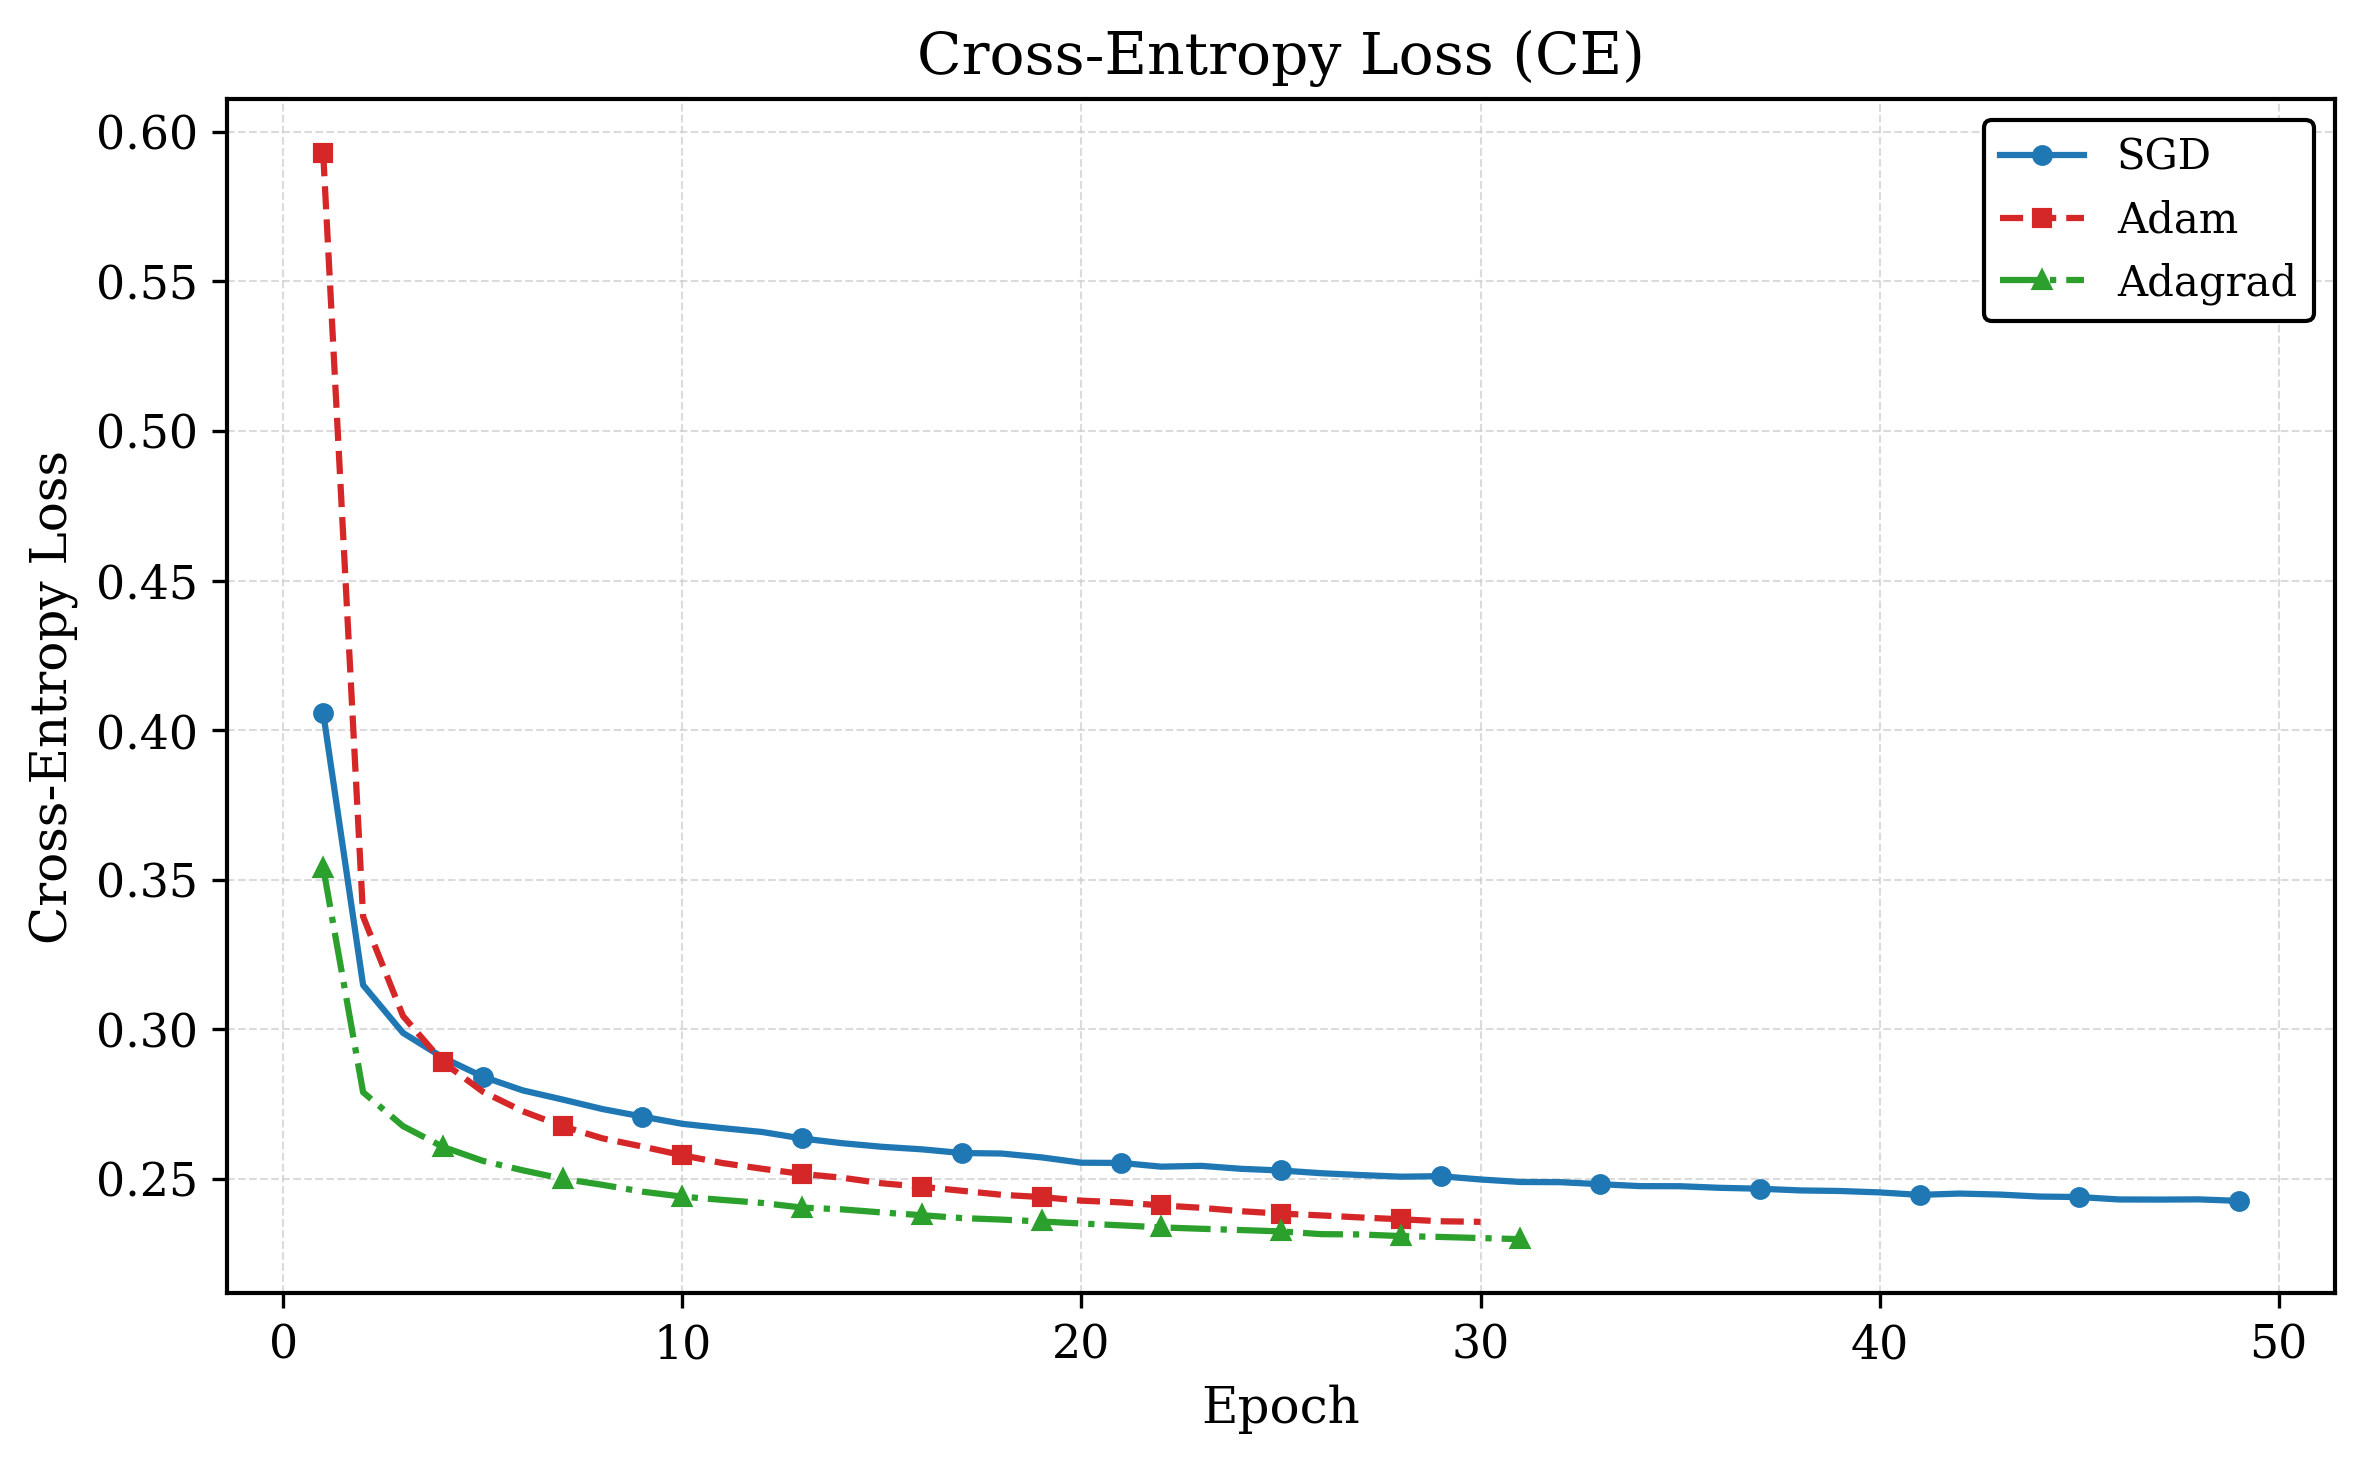
\includegraphics[width=\linewidth]{../results/ce_loss_comparison.png}
    \caption{Cross-entropy loss.}
    \label{fig:ce-loss}
\end{subfigure}
\hfill
\begin{subfigure}[b]{0.48\textwidth}
    \centering
    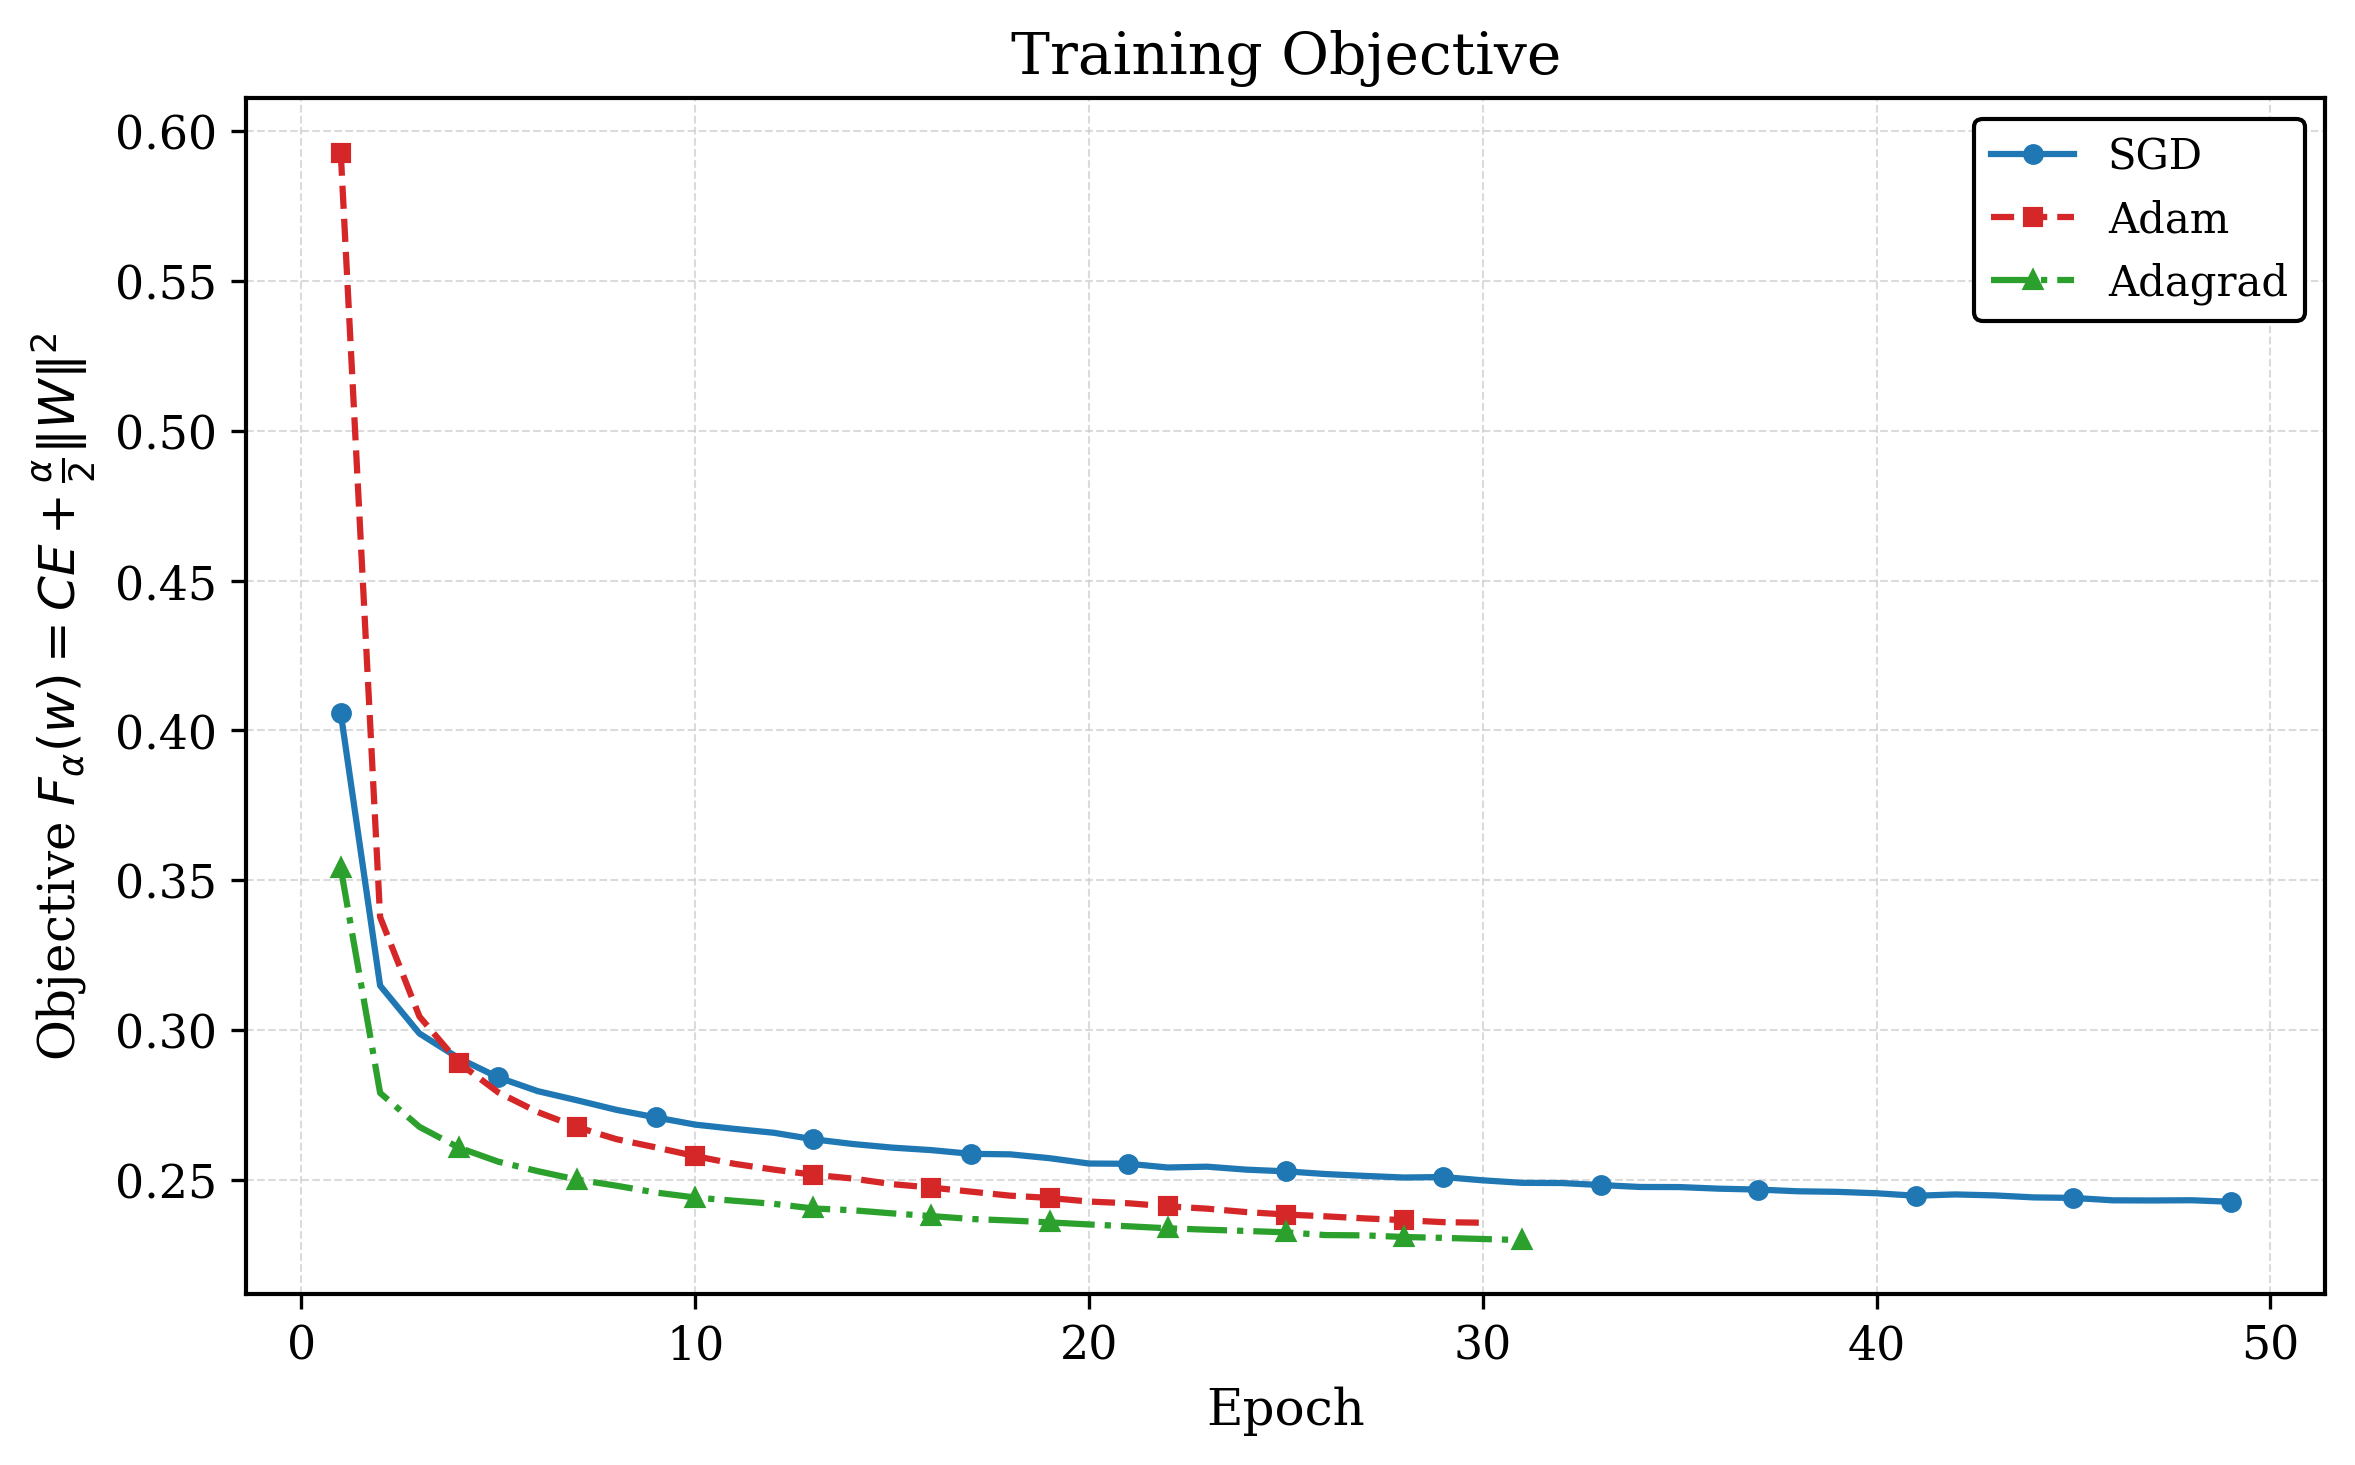
\includegraphics[width=\linewidth]{../results/obj_loss_comparison.png}
    \caption{Training objective \(F_\alpha\).}
    \label{fig:objective}
\end{subfigure}
\caption{Training dynamics: cross-entropy loss and regularized objective over epochs.}
\label{fig:loss-dynamics}
\end{figure}

\subsection{Generalization and efficiency}
Figure~\ref{fig:accuracy-dynamics} reports training and validation accuracy across epochs, along with the generalization gap (training minus validation accuracy). All three methods improve rapidly during the first epochs and then saturate near \(92\%\) validation accuracy. Training accuracy continues to increase after validation accuracy plateaus, which is expected even for a linear model with many parameters relative to the intrinsic dimension of the data. The small separation between the training and validation curves suggests moderate overfitting under the selected regularization strength. After an initial transient, the gap stabilizes around 1--2 percentage points for all methods. The negative gap at the very first epoch for Adam reflects that the model is still close to initialization and that training and validation accuracies are noisy at this stage.
\begin{figure}[H]
\centering
\begin{subfigure}[b]{0.48\textwidth}
    \centering
    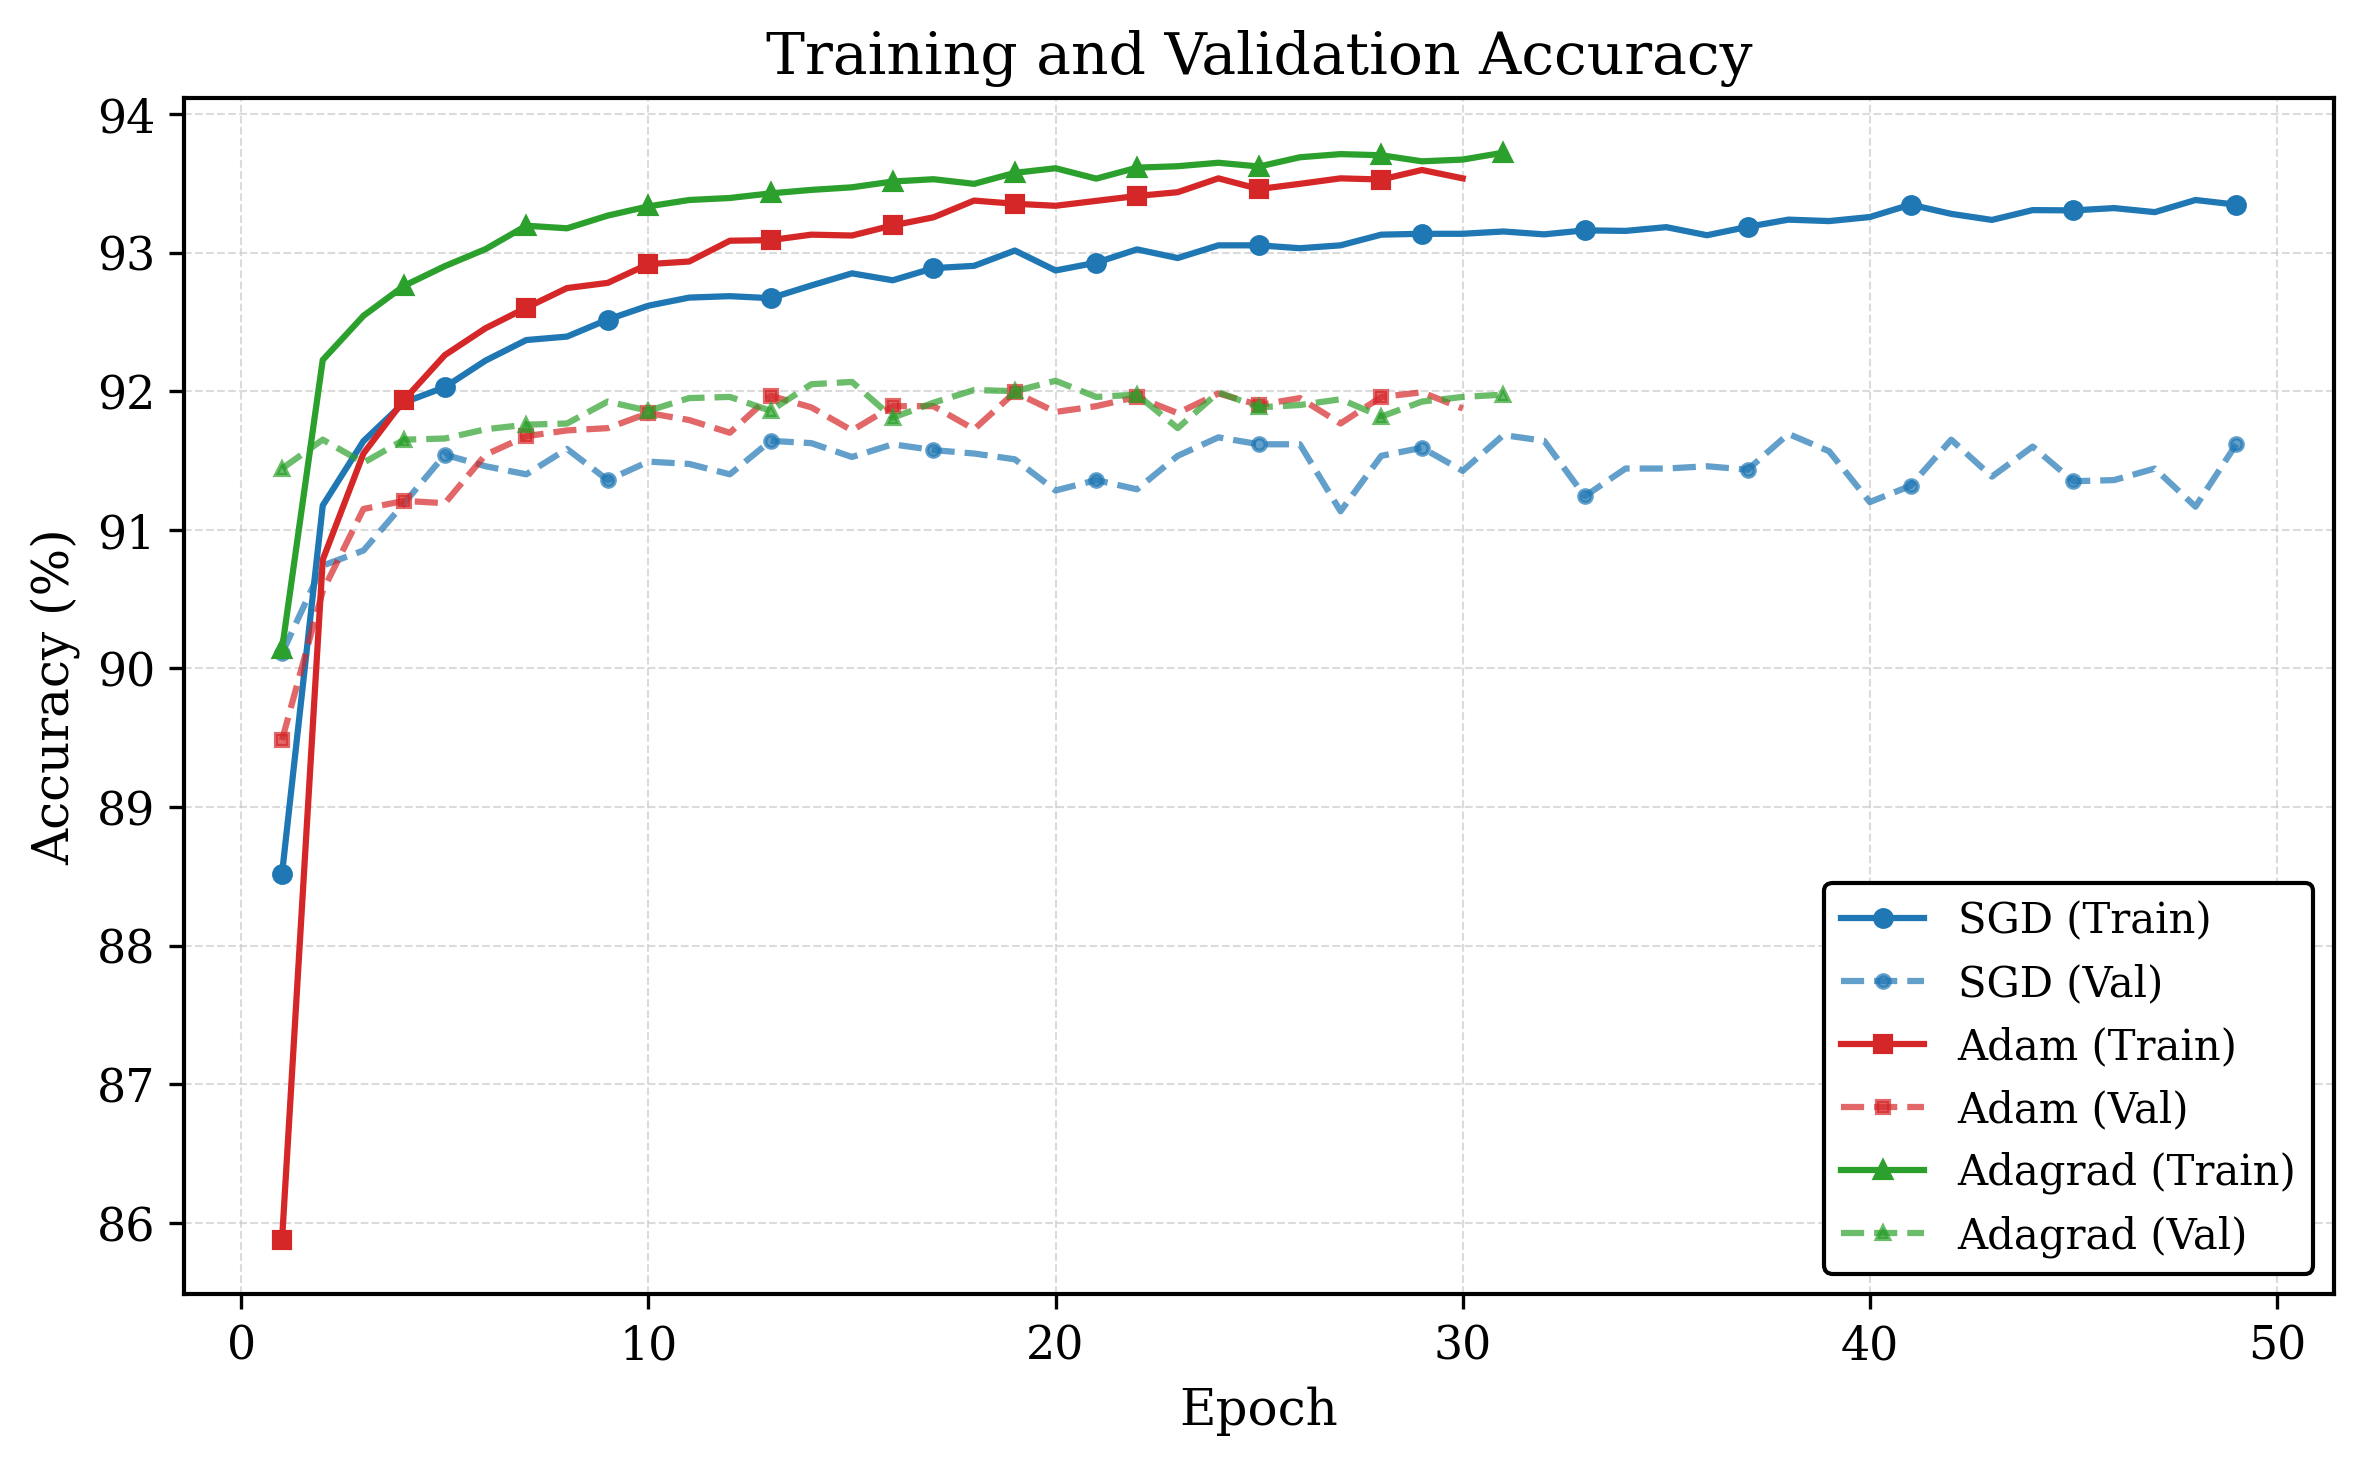
\includegraphics[width=\linewidth]{../results/accuracy_comparison.png}
    \caption{Training and validation accuracy.}
    \label{fig:accuracy}
\end{subfigure}
\hfill
\begin{subfigure}[b]{0.48\textwidth}
    \centering
    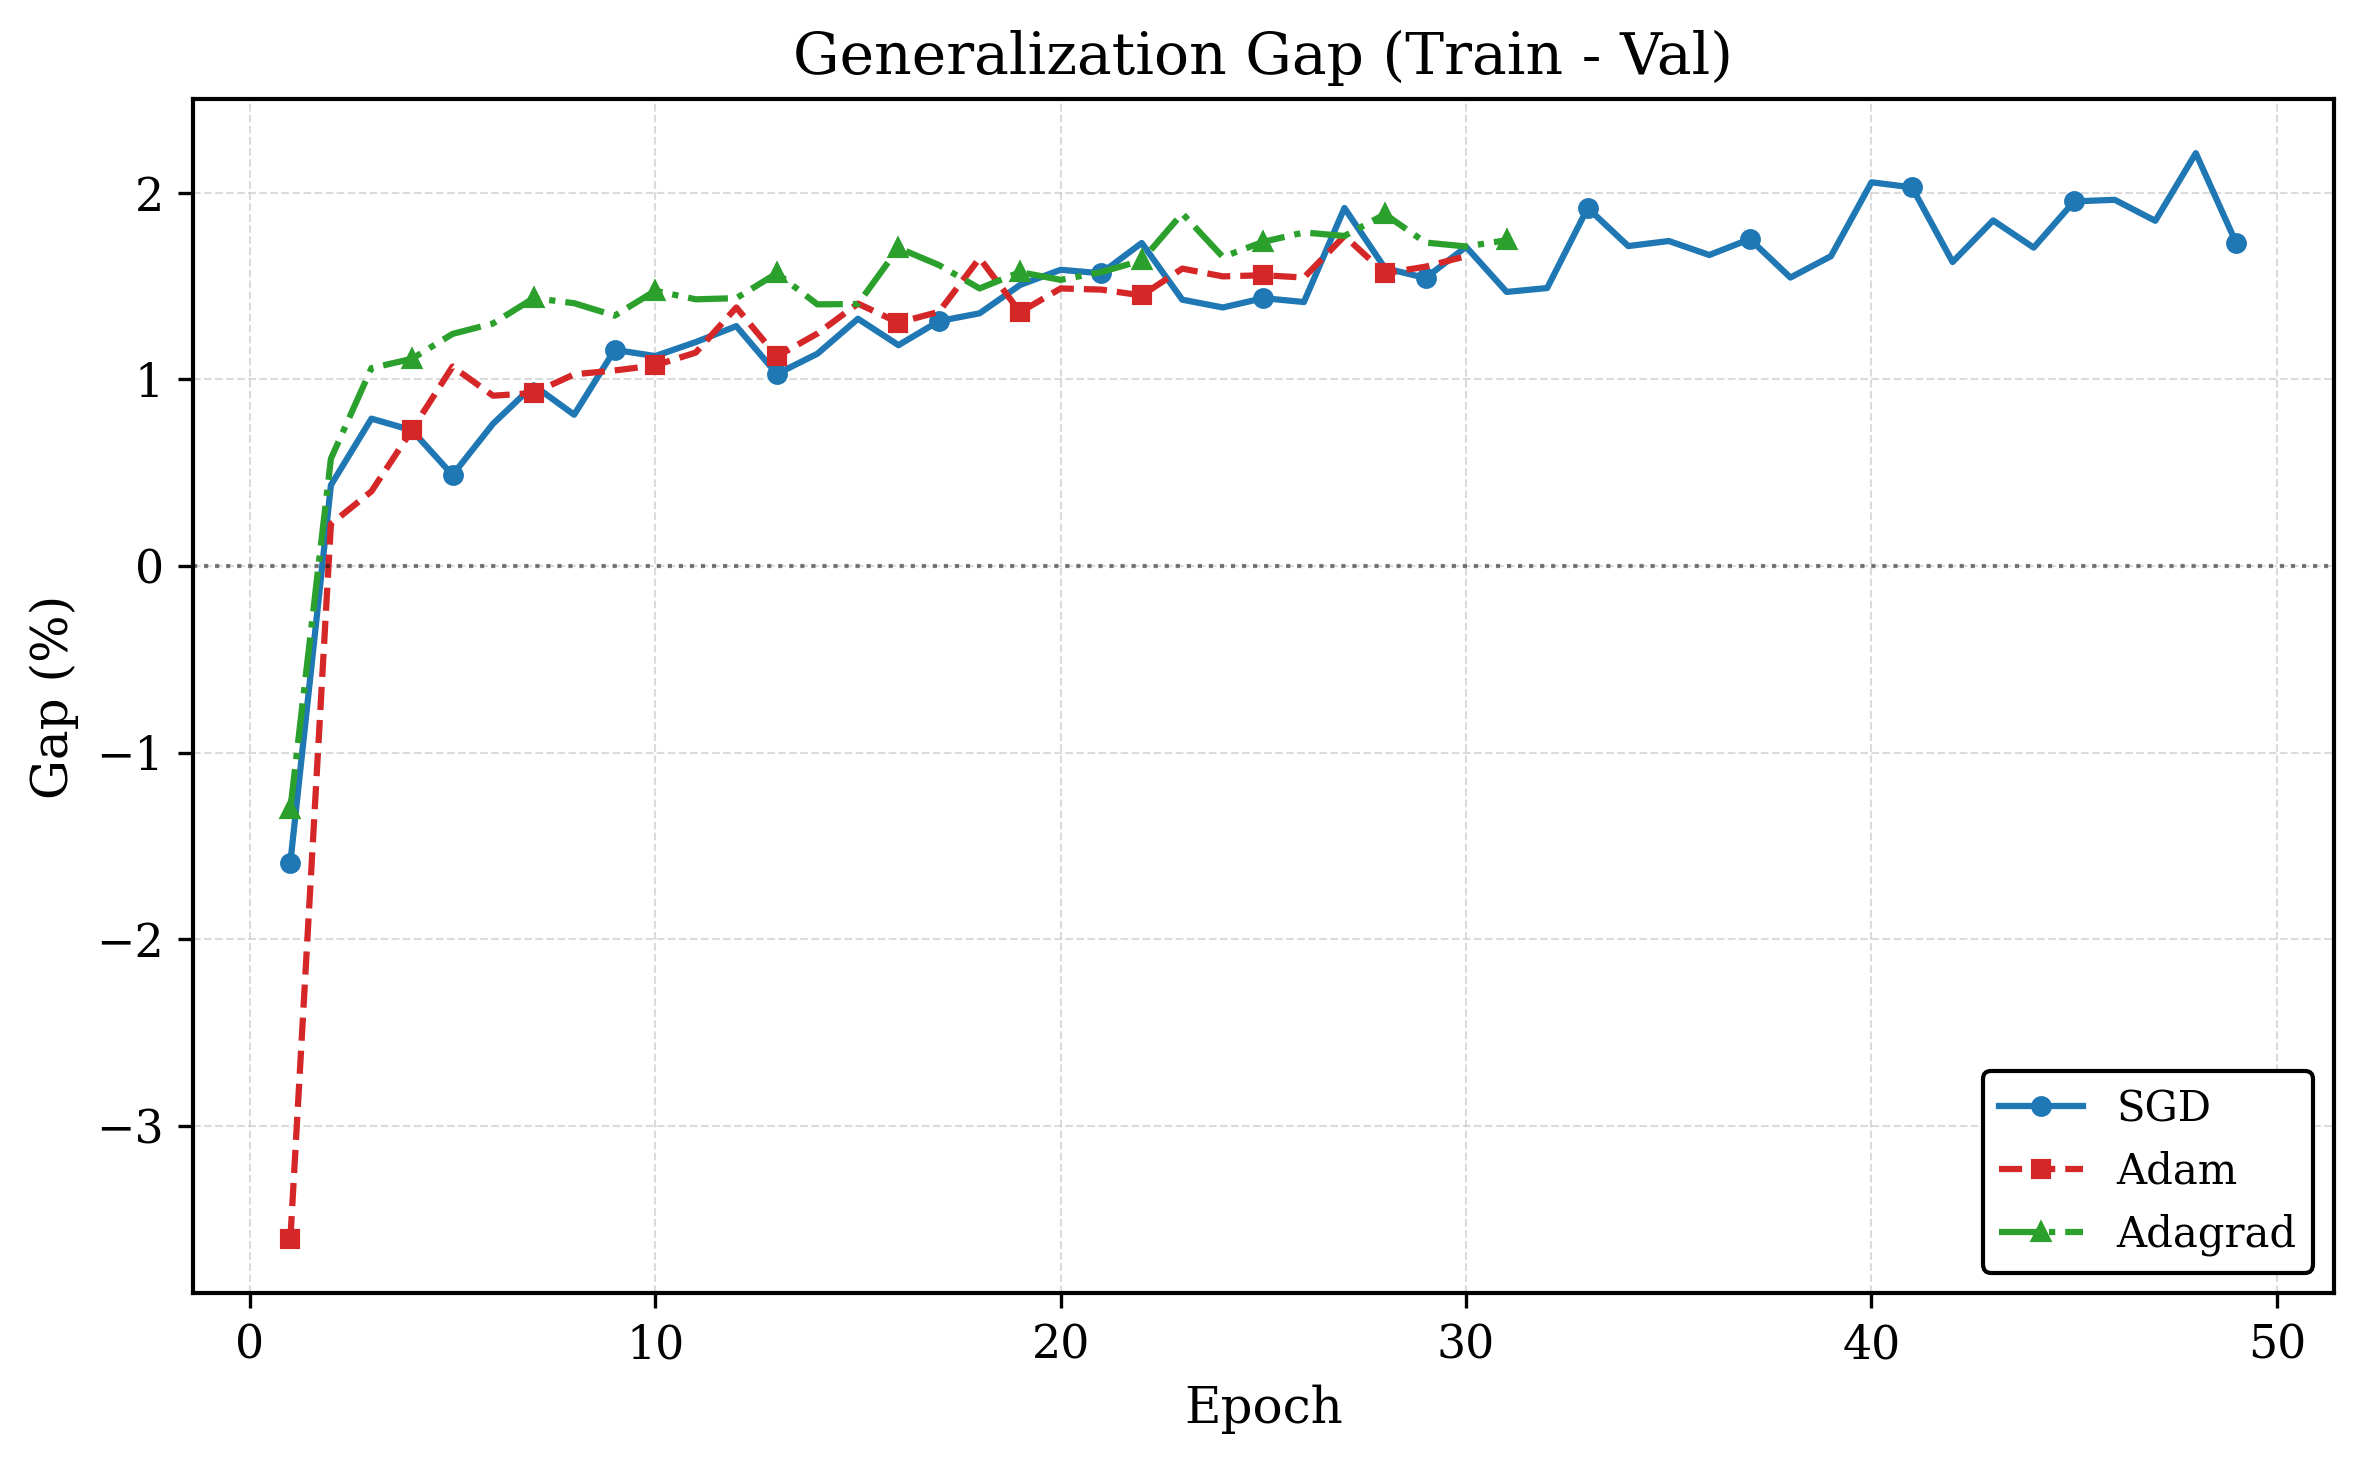
\includegraphics[width=\linewidth]{../results/generalization_gap.png}
    \caption{Generalization gap.}
    \label{fig:gap}
\end{subfigure}
\caption{Accuracy dynamics and generalization gap over epochs.}
\label{fig:accuracy-dynamics}
\end{figure}

Since the optimizers use different effective step sizes and terminate at different epochs, Figure~\ref{fig:efficiency} compares training accuracy against cumulative wall-clock time (training plus validation evaluation) and reports the norm of the recorded mini-batch gradient at the end of each epoch (log scale). We note that cumulative time includes validation evaluation and is affected by early stopping, so the total runtime also depends on stopping decisions; nevertheless, the time-to-milestone metrics in Table~\ref{tab:speed} provide a fairer comparison by measuring the time to reach fixed accuracy thresholds. Under the measured runtime, Adagrad reaches high training accuracy quickest, followed by Adam and then SGD, consistent with the loss trajectories in Figure~\ref{fig:loss-dynamics}. As discussed in Section~3, the gradient norm diagnostic is computed from the last mini-batch and is therefore noisy; it is best interpreted as a qualitative indicator of the scale of the most recent stochastic update rather than as a monotone convergence certificate.

\begin{figure}[H]
\centering
\begin{subfigure}[b]{0.48\textwidth}
    \centering
    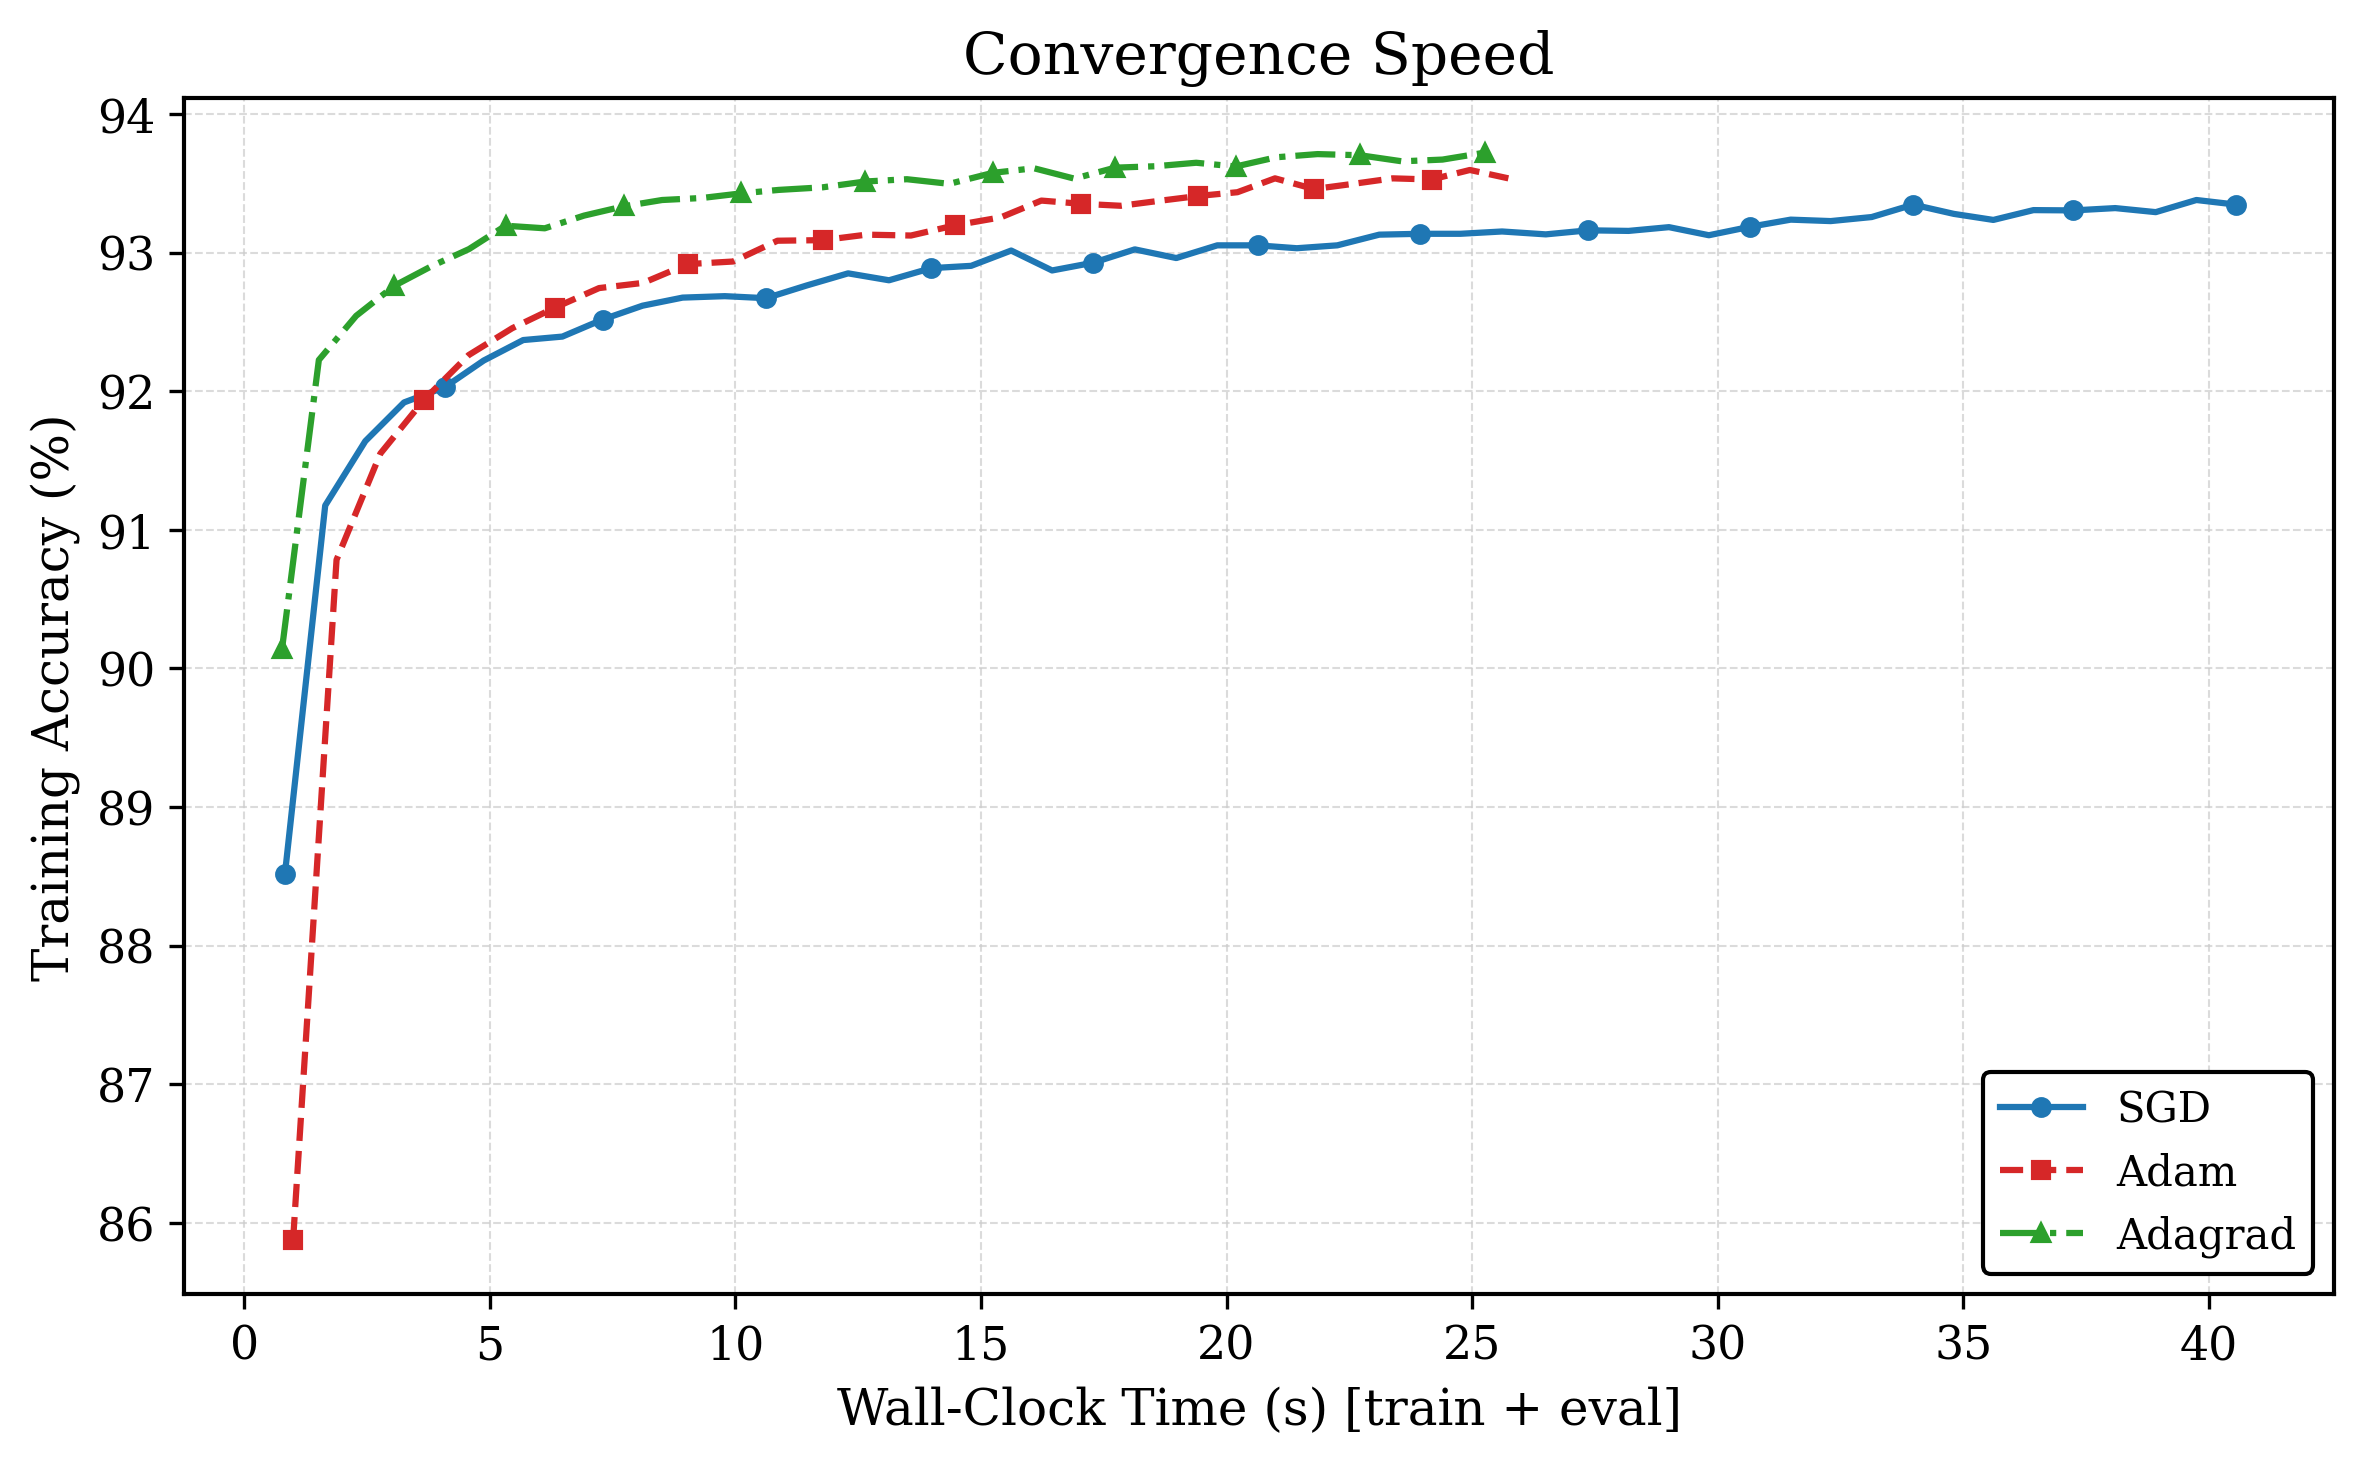
\includegraphics[width=\linewidth]{../results/time_comparison.png}
    \caption{Training accuracy versus time.}
    \label{fig:time}
\end{subfigure}
\hfill
\begin{subfigure}[b]{0.48\textwidth}
    \centering
    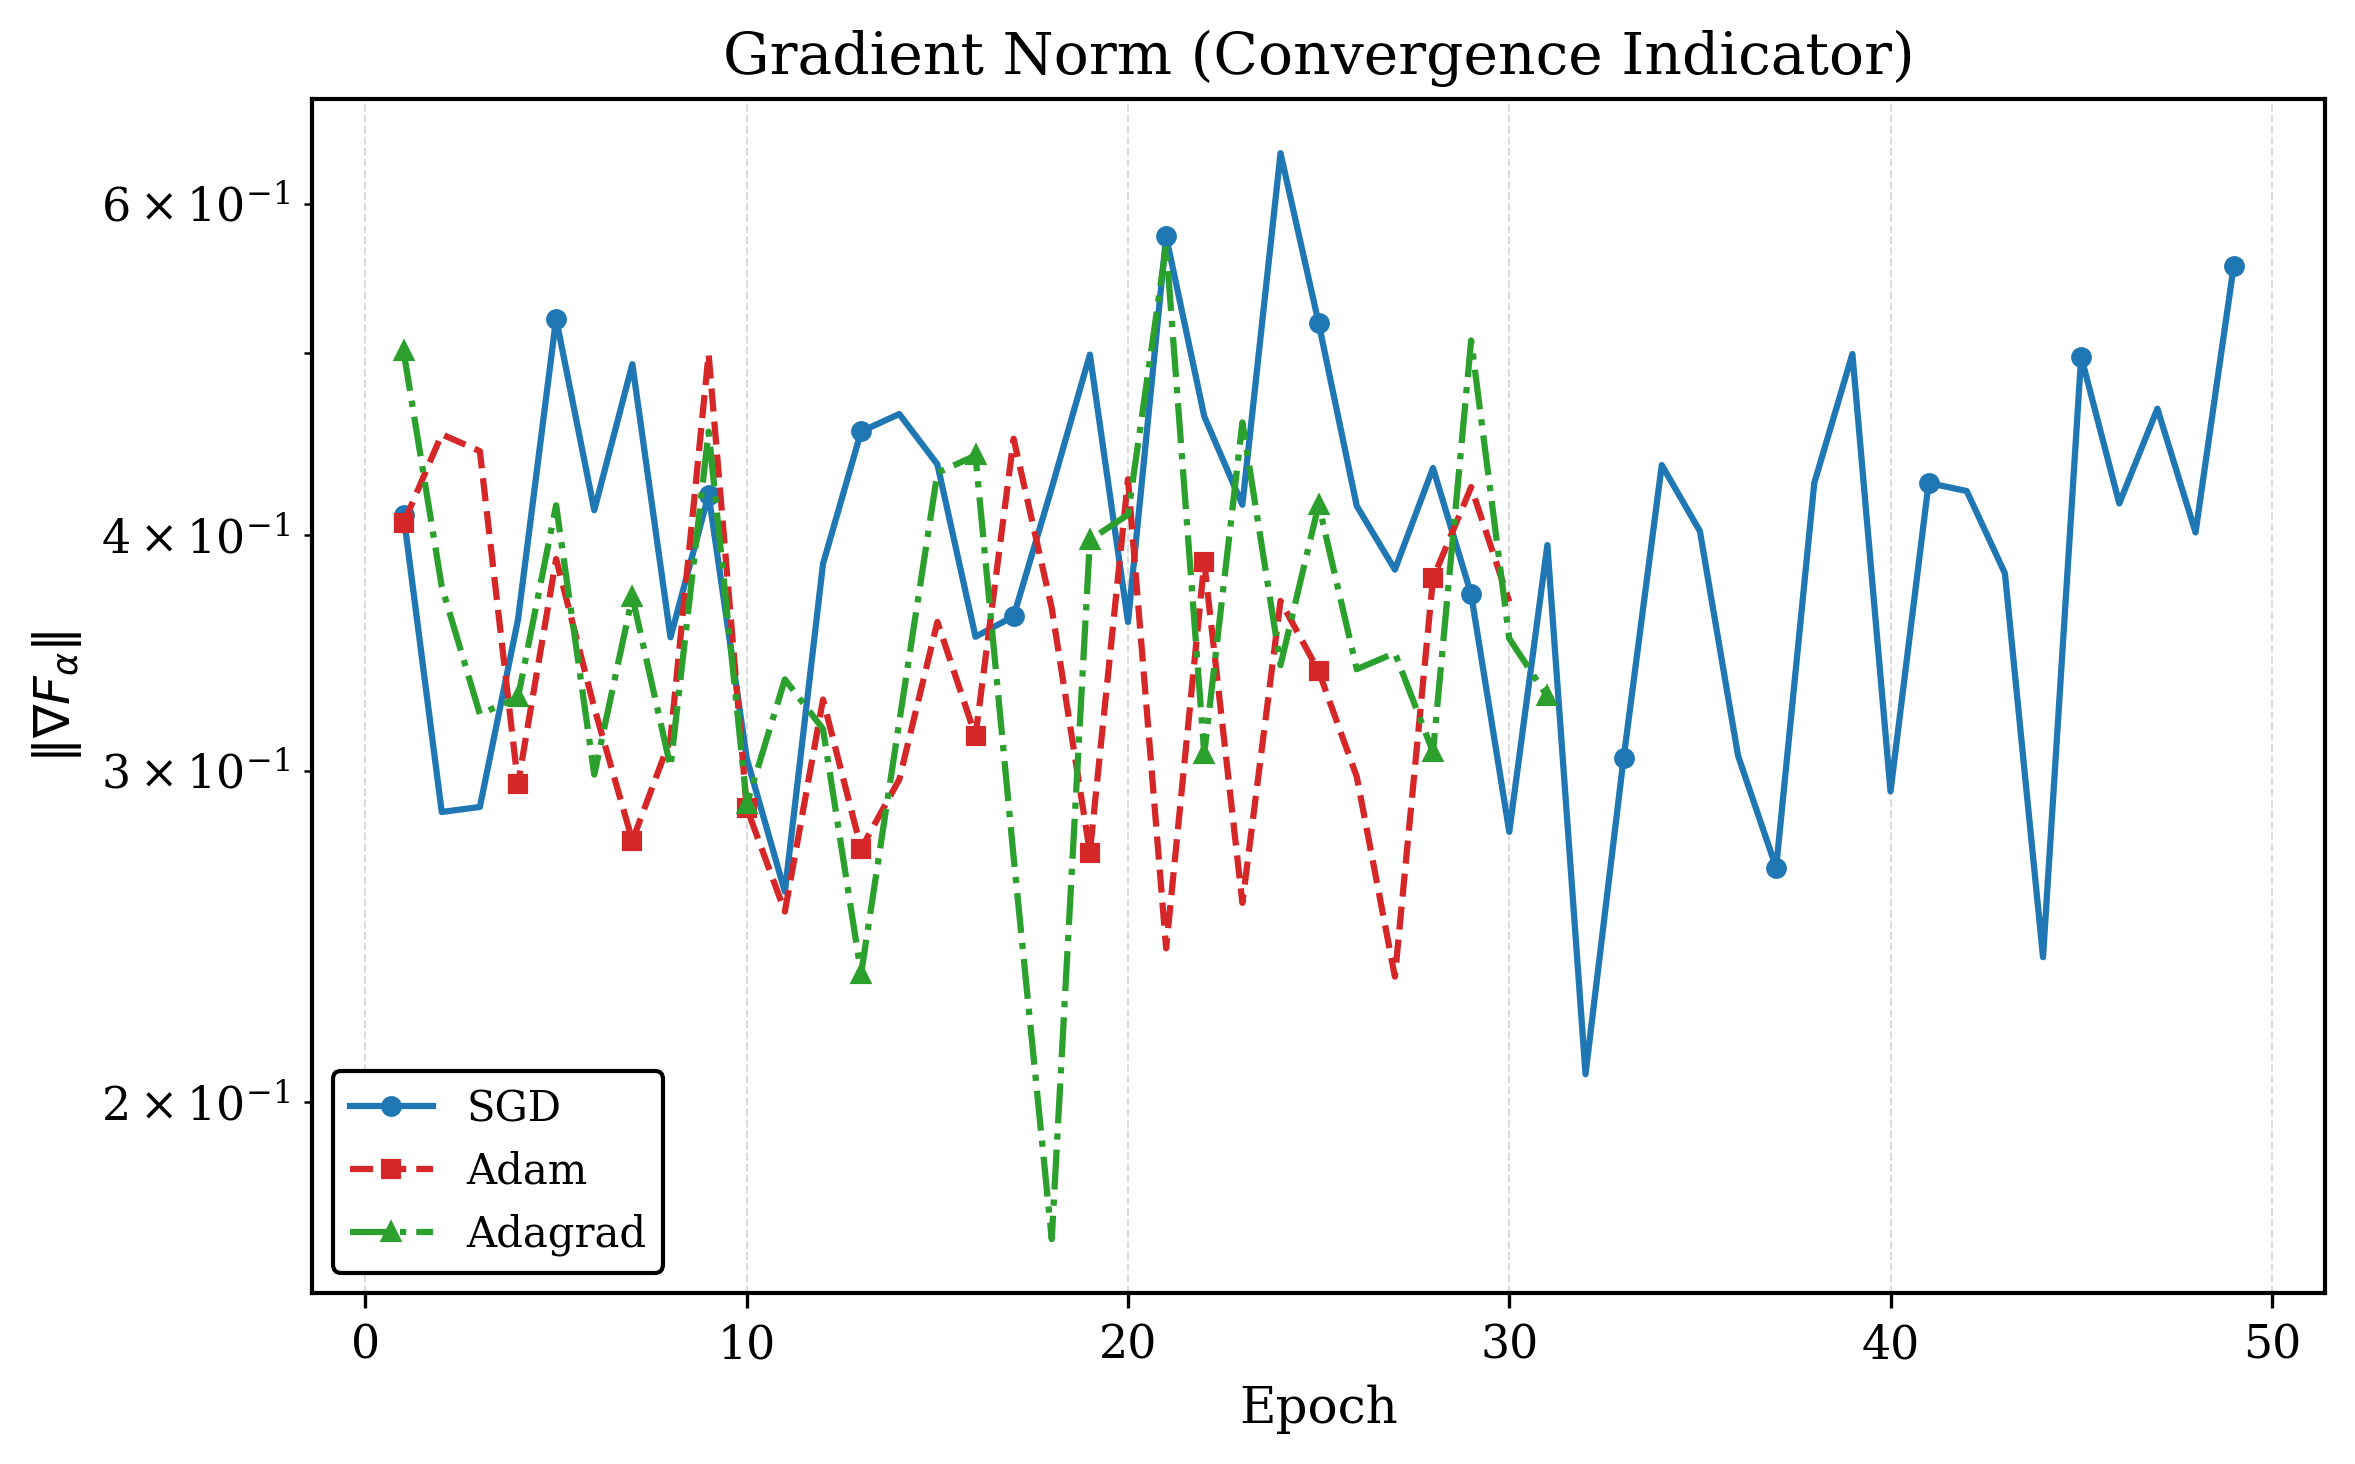
\includegraphics[width=\linewidth]{../results/gradient_norm.png}
    \caption{Mini-batch gradient norm (log scale).}
    \label{fig:gradnorm}
\end{subfigure}
\caption{Efficiency comparison: accuracy versus time and gradient norm dynamics.}
\label{fig:efficiency}
\end{figure}

To complement the time-based curve, Table~\ref{tab:speed} summarizes a few milestone times derived from the logged histories. The milestones are chosen to be attainable by all methods in this run. Adagrad reaches both milestones earlier than Adam and SGD, while SGD requires substantially more time to reach its best validation epoch.

\begin{table}[H]
\caption{Time-to-milestone summary.}
\label{tab:speed}
\centering
{\setlength{\tabcolsep}{3pt}
\begin{tabular}{@{}l>{\raggedright\arraybackslash}p{0.27\linewidth}>{\raggedright\arraybackslash}p{0.27\linewidth}>{\raggedright\arraybackslash}p{0.27\linewidth}@{}}
\toprule
\textbf{Method} & \textbf{Time to val.\(\ge 91.5\%\)} & \textbf{Time to train\(\ge 93\%\)} & \textbf{Time at best val.} \\
\midrule
SGD & \(\SI{4.09}{s}\) (epoch 5) & \(\SI{15.62}{s}\) (epoch 19) & \(\SI{31.49}{s}\) (epoch 38) \\
Adam & \(\SI{5.46}{s}\) (epoch 6) & \(\SI{10.86}{s}\) (epoch 12) & \(\SI{17.04}{s}\) (epoch 19) \\
Adagrad & \(\SI{1.52}{s}\) (epoch 2) & \(\SI{4.58}{s}\) (epoch 6) & \(\SI{16.08}{s}\) (epoch 20) \\
\bottomrule
\end{tabular}
}
\end{table}

Several limitations remain. First, only training and validation performance are reported; evaluation on the official MNIST test set would provide a more standard benchmark. Second, the tuning and early-stopping procedures trade computational cost for optimization accuracy; different budgets or stopping rules may change the selected hyperparameters. Third, the reported differences between Adam and Adagrad are small in validation accuracy under a single seed, so repeated runs would be necessary to assess variability and statistical significance.

\section{Conclusion}
This report investigated stochastic optimization methods for multinomial logistic regression on the MNIST digit classification task. The main contributions and findings are summarized as follows:

\begin{itemize}
    \item \textbf{Problem Formulation.} We formulated the classification task as a convex empirical risk minimization problem with optional \(\ell_2\) regularization, expressed through the objective function \(F_\alpha(W)\). The bias-free multinomial logistic regression model with \(7{,}840\) trainable parameters provides a tractable yet representative setting for comparing stochastic optimization algorithms.
    
    \item \textbf{Gradient Derivation.} We derived the gradient and stochastic gradient expressions in both per-class vector form and compact matrix form. The per-class gradient \(\nabla_{w_j}\ell_i(W) = (p_j(x_i;W) - y_{i,j})x_i\) has a clear probabilistic interpretation, and the matrix formulation \(\nabla_{W^\top} = \frac{1}{|B|}(P_B - Y_B)^\top X_B\) enables efficient mini-batch computation. The derived formulas were verified for dimensional consistency and directly linked to the implementation.
    
    \item \textbf{Algorithm Comparison.} Three stochastic first-order methods---SGD, Adagrad, and Adam---were compared under a unified experimental protocol with two-stage hyperparameter tuning and validation early stopping. Among these:
    \begin{itemize}
        \item Adagrad achieved the highest validation accuracy (\(92.08\%\)) and reached accuracy milestones in the shortest wall-clock time, benefiting from its coordinate-wise adaptive step sizes.
        \item Adam achieved nearly identical validation accuracy (\(91.99\%\)) with comparable runtime, demonstrating the effectiveness of combining momentum with adaptive normalization.
        \item SGD achieved slightly lower validation accuracy (\(91.69\%\)) and required more wall-clock time, reflecting its sensitivity to step-size selection in the absence of adaptation.
    \end{itemize}
    
    \item \textbf{Regularization Analysis.} The hyperparameter search indicated that \(\alpha = 0\) (no explicit regularization) yielded the best validation performance for all three methods under this protocol. Increasing \(\alpha\) consistently degraded validation accuracy, suggesting that the model capacity is well-matched to the task and that implicit regularization from early stopping suffices.
    
    \item \textbf{Convergence Behavior.} All methods exhibited rapid initial improvement followed by saturation near \(92\%\) validation accuracy. The generalization gap (training minus validation accuracy) stabilized at 1--2 percentage points, indicating moderate overfitting that did not substantially affect the ranking of methods.
\end{itemize}

\end{document}

